\documentclass{beamer}
%\documentclass[notes=show]{beamer}

\usepackage[utf8]{inputenc}
\usepackage[ngerman]{babel}
\usepackage{rotating}
\usepackage{float}
\usepackage{subfigure}

\usepackage{latexsym}
\usepackage{floatflt}
\usepackage{graphicx}
%\definecolor{lightblue}{rgb}{0.8,0.9,1.0}
%\usetheme{PaloAlto}
%\usetheme{Darmstadt}
\usetheme{Frankfurt}
%\usetheme{Berlin}

%\usecolortheme{crane}
%\usecolortheme{wolverine}
\usecolortheme{seagull}
%\usecolortheme{albatross}
%\usecolortheme{beetle}
%\usecolortheme{lily}

\usepackage{pgf,pgfarrows,pgfnodes,pgfautomata,pgfheaps}
\usepackage{amsmath,amssymb}

\setbeamercovered{dynamic}


%notes:
\setbeamertemplate{note page}[plain] 
%compressed

\title[]{  Simulation paralleler E/A auf \\ Anwendungs- und Systemebene }
\author{ \underline{Julian M. Kunkel} } %Research Group:
\institute{ Institut für Informatik \\  Parallele und Verteilte Systeme \\ Ruprecht-Karls-Universit\"at Heidelberg}
\date{  28.09.2009 }
\beamertemplatetransparentcovereddynamic
\setbeamerfont{note page}{size=\small}
%\setbeamersize{text margin left=0.1cm,text margin right=0.1cm}
%\renewcommand{\>}{\rangle}
%\newcommand{\<}{\langle} 
%\usebeamercolor[fg]{[page number]}

\setbeamertemplate{navigation symbols}{}
%\setbeamertemplate{note page}{}

\setbeamersize{text margin left=0.2cm}
\setbeamersize{text margin right=0.2cm}
\setbeamersize{sidebar width right=0cm}
\setbeamersize{sidebar width left=0cm}

\setbeamertemplate{footline}
{
\begin{beamercolorbox}{title}
\hspace*{0.2cm}
% \copyright 
Julian M. Kunkel 
\hfill
 \insertslidenavigationsymbol
 \insertframenavigationsymbol
 \insertsubsectionnavigationsymbol
 \insertsectionnavigationsymbol
 \insertdocnavigationsymbol
 \insertbackfindforwardnavigationsymbol
 \hfill\insertframenumber/\inserttotalframenumber
 \hspace*{0.2cm}
\end{beamercolorbox}
}

%\newcommand{\markNote}[1]{	\textsuperscript{\tiny [#1]} }
\newcommand{\markNote}[1]{	 }

%\AtBeginSection[]{
%\frame{
      %\frametitle{Outline}
	%\tableofcontents[current,hideallsubsections]
%	}
%}

\begin{document}
\frame{
	\titlepage
}

\frame{
\frametitle{Agenda}
\tableofcontents[hideallsubsections]
}

\newcommand {\myframe}[2]{
\frame{
	\frametitle{#1} 
	\begin{itemize}
	#2 
	\end{itemize}
}
}

\newcommand {\itemm}[1]{
  	\begin{itemize}
	\item #1
	\end{itemize}
}

\section{Ziele}

\myframe{Ziele}{
\item MPI and MPI-IO Befehle simulieren
  \itemm{Abschätzung für Effizienz einer Implementierung}
\item Einfache Modelle für Hardware und Software
\item Konfiguration der Hardware/Software nach belieben
  \itemm{Schätze Skalierbarkeit von Algorithmus in beliebigen Cluster Umgebungen}
\item Einsatz/Nutzbarmachung von Standard-Tools zur Analyse
  \itemm{Simulationsergebnisse genau wie realle Programläufe bewerten}
\item Neue Algorithmen/Verhalten schnell und reproduzierbar testen
\item Einsetzbarkeit für Lehre
   \itemm{Soll auf Desktop PC lauffähig sein}
}

\section{Hardware Model}
\subsection{Hardware Modell}
\myframe{Hardware Modell}{
\item Komponententypen an existierende Hardware angelehnt\\ z.B. “Knoten” oder “I/O-subsystem”
\item Je Komponententyp sind alternative Implementierungen möglich\\ z.B. SSD oder Disk
\item Cluster Modell beschreibt konkrete Implementierungen der Komponenten und Charakteristika
\item Deterministisches Komponentenverhalten
}

\subsection{Simulierte Komponenten}
\frame{
  \frametitle{Simulierte Komponenten}
  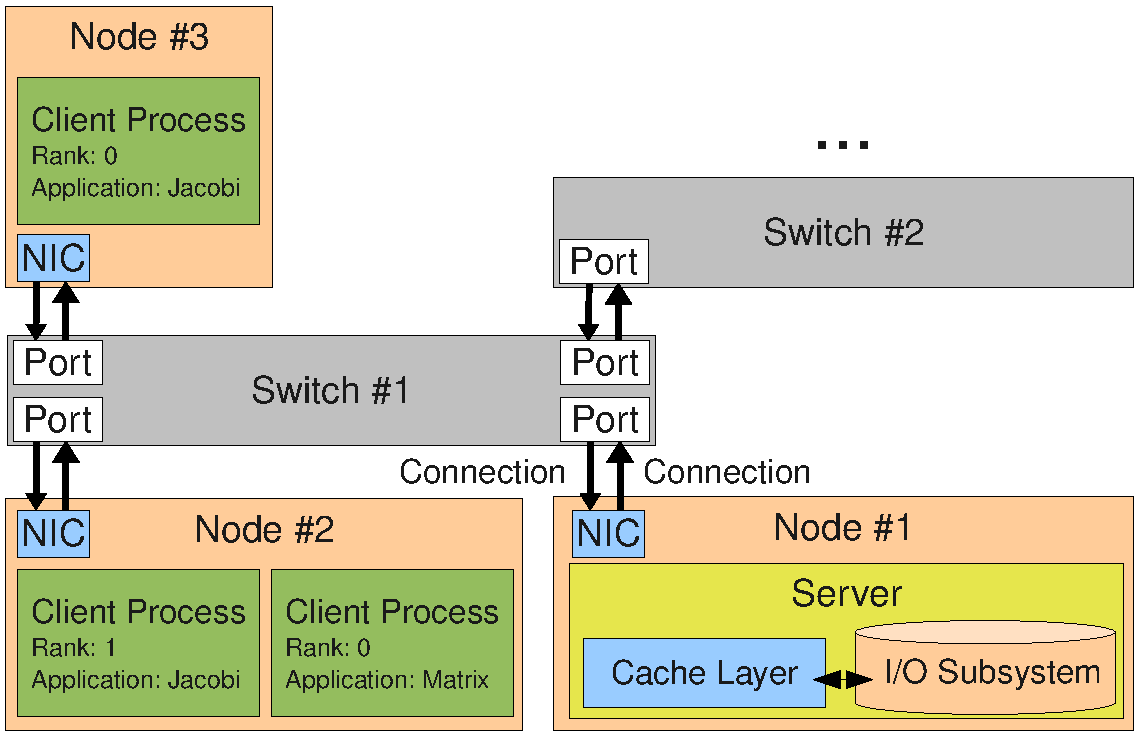
\includegraphics[width=0.95\textwidth]{Simulator-Components.pdf}
}

\subsection{Hardware Model - Charakteristika}
\myframe{Hardware Model - Charakteristika}{
\item Knoten:
  \itemm{\# CPUs, Abarbeitungsgeschwindigkeit}
\item Netzwerkkarte:
  \itemm{Latenz, Durchsatz}
\item Server Cache Layer:
\itemm{Cache Größe, Algorithmus}
\item I/O Subsystem:
\itemm {Letzter Zugriff (Datei, Offset) bestimmt Zugriffszeit
    \item Track-To-Track Zugriffzeit, Mittlere Zugriffszeit}
\item Switch:
  \itemm{Store-and-Forward Switching
  \item Besteht aus N-Ports}
\item Port:
  \itemm{Latenz, Durchsatz}
}

\subsection{Netzwerk Datenfluss Model}
\myframe{Datenfluss Model}{
  \item Datenflüsse als Flüsse von Paketen (Transfer Granularität)
  \item Datenfluss Model ist an Realität angelehnt garantiert aber optimalen Transfer (unter gegegebener Granularität) 
  \item Server können Datenflüsse aktiv blockieren z.B. bei gefülltem I/O Cache 
  \item Überholvorgänge innerhalb des Netzwerks sind nicht möglich
  \item Gegenwärtig nur eine Route
} 

\myframe{Paketübertragung}{
  \item Eine Netzwerkkomponente kann eine Menge von Paketen transferieren 
  \itemm{Bis das Kabel mit Daten saturiert ist
    \item Der weitere Datenfluss wird dann blockiert} 
  %\item Alternative Anschauung: wenn mindestens soviele Daten unterwegs sind um die Latenz zu überbrücken 
  \item Bei Bearbeitung eines Pakets wird der Sender benachrichtigt
    \itemm{Diese darf nun weitere Pakete transferieren 
    \item Kaskade von nachrückenden Paketen kann aktiviert werden}
  \item Es wird ein Fluss pro Ziel nach obigem Schema verwaltet
   \itemm{Engpässe die in Flussrichtung auftreten blockieren nicht den Transfer an andere Adressen
     \item Anschaulich: ein Switch verwaltet pro Netzwerkadresse eine Warteschlange mit fester Länge
   }
}

\section{Software Model}
\subsection{Software Model}
\myframe{Software Model}{
\item Anwendung 
\itemm{MPI Semantik
  \item Nichtblockierende Operationen werden unterstützt
  \item Rechenoperationen werden nur durch eine Dauer charakterisiert
  \item Gleichmäßige Zuteilung der CPU Ressourcen zu Rechenjobs}
  
\item Mehrere (MPI-IO) Anwendungen können gleichzeitig gestartet werden  
  \itemm{Insbesondere im I/O-Subsystem ist ein anderes Lastverhalten zu erwarten}
}

\subsection{Modellierung von MPI Befehlen}
\myframe{Modellierung von MPI Befehlen}{
  \item Algorithmen sind austauschbar
  \itemm{Bei Ausführung Algorithmus spezifizieren}
\item Abarbeitung in endlichen Automaten
  \itemm{Programmierung der Zustände
    \item Existierende Befehle können aufgerufen werden
    \item Netzwerkoperationen 
    \item (Eigenverwaltete) Blockierung möglich}
\item Globale Sicht auf alle Prozesse 
  \itemm{Metawissen soll Programmierung von einem Best-Case erlauben
    \item Ermöglicht bspw. “Virtuelle” Bariere}
}

\section{Implementierung}
\myframe{Implementierung des Simulators}{
  \item Java (Version 5)
  \item GPL
  \item Sequenzieller Code
  \item Schreibt TAU-Trace oder HDTrace zur Analyse
  \begin{block}{Diskrete Ereignis-Simulation}
  Solange Ereignisse vorhanden sind:
  \itemm{    
    Bearbeite (ein) frühestes Ereignis durch delegation an zuständige Komponente
    \item Erzeugt ggf. weitere Ereignisse in der Zukunft
    }
  \end{block}

\begin{block}{Job == Auftrag - durch blockierende Verarbeitung realisiert}
    \begin{itemize}
     \item Start und Ende Ereignis
     \item Beispiel: Datenpakete werden durch Store-and-forward weitergeleitet
     \item Bearbeitung von Jobs wird von Komponenten selbstverwaltet (meist FIFO)
    \end{itemize}   
  \end{block}
}

\section{Ergebnisse}
\subsection{Validierung des Simulators}
\myframe{Validierung des Simulators}{
 \item Existierender Program getraced und simuliert
 \item Jacobi Verfahren - PDE: Iterative Lösung der Poisson Gleichung
 \itemm{
 100 Iterationen
 \item Master Prozess sammelt Ergebnisse ein
 \item Keine I/O 
 }
 \item Cluster Model analog zu unserem 10 Knoten (Test-)Cluster
}

\frame{
  \frametitle{Jacobi - PDE}
   
\begin{table}
\begin{center}
\begin{tabular}{l||l|l|l}
Prozessanzahl & Laufzeit in s & Simulierte Laufzeit & Simuliert/Real \\
\hline
\hline
1 & 47.30 & 47.35 & 1.001 \\
2 & 24.79 & 24.93 & 1.006 \\
3 & 17.3 & 17.54 & 1.014 \\
4 & 13.54 & 13.75 & 1.016 \\
5 & 11.56 & 11.82 & 1.022 \\
6 & 10.09 & 10.33 & 1.024 \\
7 & 9.16 & 9.44 & 1.030 \\
8 & 8.39 & 8.73 & 1.041 \\
9 & 8.00 & 8.26 & 1.033
\end{tabular}
\end{center}
\end{table}

}

\subsection{Evaluation von I/O Optimierungen}

\myframe{Evaluation von I/O Optimierungen}{
  \begin{block}{Ziele}
  \item Effizienz verschiedener Optimierungen soll überprüft werden
  \item Kollektive Optimierungen - Two-Phase* vs. serverseitige Optimierungen
  \item Entwicklung neuer I/O Optimierungsstrategien
  \end{block}
}

\frame{
\frametitle{Serverseitige Optimierungen}
\begin{block}{Stand der Technik}
  \begin{itemize}
   \item I/O Zugriffe werden von Betriebsystem optimiert
   \itemm{Betriebsystem Cache und Write-Behind} 
   \item Typischerweise maximale Anzahl an Operationen die ans Betriebsystem gegeben werden
   \itemm{Cluster Dateisystem trifft Vorauswahl, wann - welche I/O-Operationen}
   \item $\Rightarrow$ Die I/O Schicht verfügt nur über Teilwissen der I/O Anfragen
   \item Bei Lesezugriffen ist die Reihenfolge entscheident um Random-Access zu verhindern
   \item Bei Schreibzugriffen nicht so gravierend, da Write-Behind Optimierungen erlaubt   
  \end{itemize}
\end{block}
}

\frame{
\frametitle{Server-Directed I/O}
  \begin{block}{Theorie}
  \begin{itemize}
  \item Cache-Optimierungsstrategie auf I/O Servern
  \item Datentransfer zwischen Client/Server wird durch Server bestimmt
  \itemm{Interessant für Nichtzusammenhängende Zugriffe
    \item Geht über Kernel Optimierungen hinaus, da alle Anfragen berücksichtigt
    }    
  \item Der Server kennt seine eigenen I/O-Charakteristika am besten
  \end{itemize}  
  \end{block}
  
  \begin{block}{Umsetzung im Simulator}
  \begin{itemize}
  \item Cache-Schicht aggregiere Zugriffe (AggregationCache)
    \itemm{Nutze Wissen über Anfragen}
  \item Erweiterung sortiert auch die Zugriffe um (Server-Directed)
    \itemm{Nutze Wissen über I/O-Subsystem Charakteristika}
  \item Im Moment wird Datentransfer nur bei lesenden Zugriffen angepasst
    \itemm{Write-Behind erlaubt schon sehr gute Aggregationen
    \item Optional kann man Data-Sieving noch in Cache Schicht einbauen}
  \end{itemize}
  \end{block}
}

\frame{
\frametitle{Evaluation}

\begin{block}{Simuliertes Cluster}
\begin{itemize}
  \item 10 Clients, Zugriffsmuster Simple-Strided [1,2,...,10,1,2,...,10]
  \item 10 Server
    \itemm{ 
      1000\,MB Cache (RAM)
      \item Platte - 50\,MB/s, 10\,ms mittlere Zugriffszeit, track-to-track 1\,ms
      \itemm{bis 5\,MByte track-to-track seek sonst mittlerer Zugriff}
    }
  \item Sternförmige Vernetzung
  \itemm{Netzwerkkarten -- Durchsatz 100\,MB/s, Latenz 0.2\,ms
    \item Switch Durchsatz limitiert auf 1000\,MB/s
  }
  \item Datenverteilung: Stripping mit 64\,KByte
\end{itemize}
\end{block}
}

\frame{

\begin{block}{Experimente}
 Sequenzielle E/A einer Datei mit 1000\,MByte
 \begin{itemize}
  \item Unabhängige I/O mit einem, 100 oder alle Blöcke 
  \item Two-Phase
  \item Interleaved Two-Phase 
  \end{itemize}
\end{block}

  \begin{block}{Erwartungen}
  \begin{itemize}
   \item Flaschenhals sind die Festplatten
   \item Maximal 50\,MB/s pro Client und Server
   \item Two-Phase weniger als 50\,MB/s wegen Netzwerktransport
   \end{itemize}
  \end{block}
}

\frame{
\frametitle{Vergleich von Optimierungsstrategien, Blockgröße: 5\,KB}
\begin{center}
\begin{figure}
  \subfigure{
        \includegraphics[width=0.95\textwidth]{images/Overview-5K-Read.pdf}                                    
   }
   \subfigure{
        \includegraphics[width=0.95\textwidth]{images/Overview-5K-Write.pdf}            
   }
\end{figure}                                                                                    
\end{center}                                                                           
}

\frame{
\frametitle{Vergleich von Optimierungsstrategien, Blockgröße: 512\,KB}
\begin{center}
\begin{figure}
  \subfigure{
        \includegraphics[width=0.95\textwidth]{images/Overview-512K-Read.pdf}                                    
   }
   \subfigure{
        \includegraphics[width=0.95\textwidth]{images/Overview-512K-Write.pdf}            
   }
\end{figure}                                                                                    
\end{center}                                                                           
}

\frame{

Warum ist ServerDirected bei lesendem Zugriff teilweise so langsam?
\begin{block}{Analyse}
 \begin{itemize}
  \item Problemfall: Blockgröße 5\,KByte
  \item Bei individueller I/O nur 1\,MB/s
  \item Beim nicht zusammenhängendem Zugriff mit 100 Blöcken nur 15\,MB/s
  \item Mit Viewer Simulationsergebnisse betrachten
  \item Im folgenden gekürzte (und beschriftete) Screenshots
  \itemm{Nur ein Teil der Server und Clients gezeigt}
 \end{itemize}
\end{block}
}

\frame{
\frametitle{Unabhängige zusammenhängende I/O - 5\,KB - Startphase}
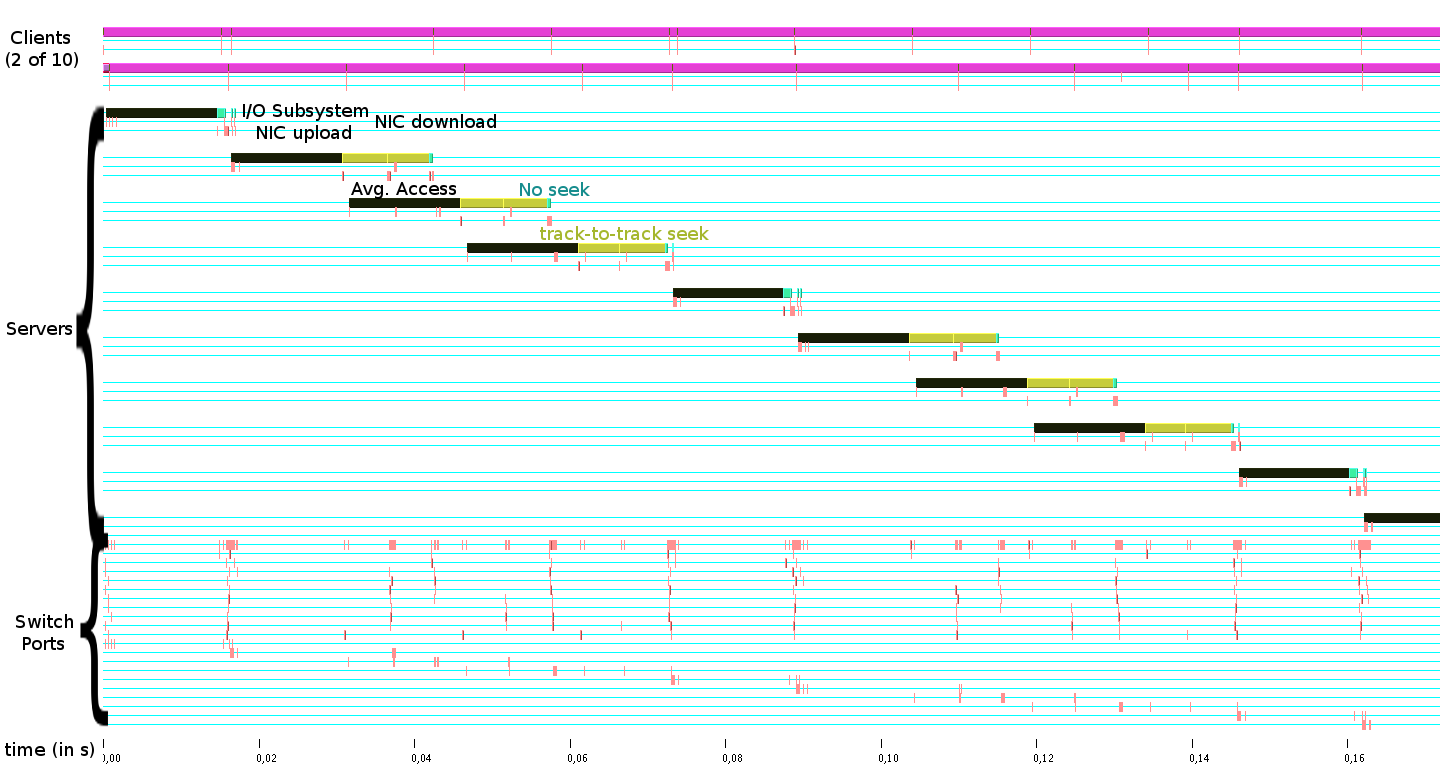
\includegraphics[width=\textwidth]{images/Screenshot-IndividualStartup-5KB-1OpPerIteration.png}
}

\frame{
\frametitle{Unabhängige zusammenhängende I/O - 5\,KB - Später}
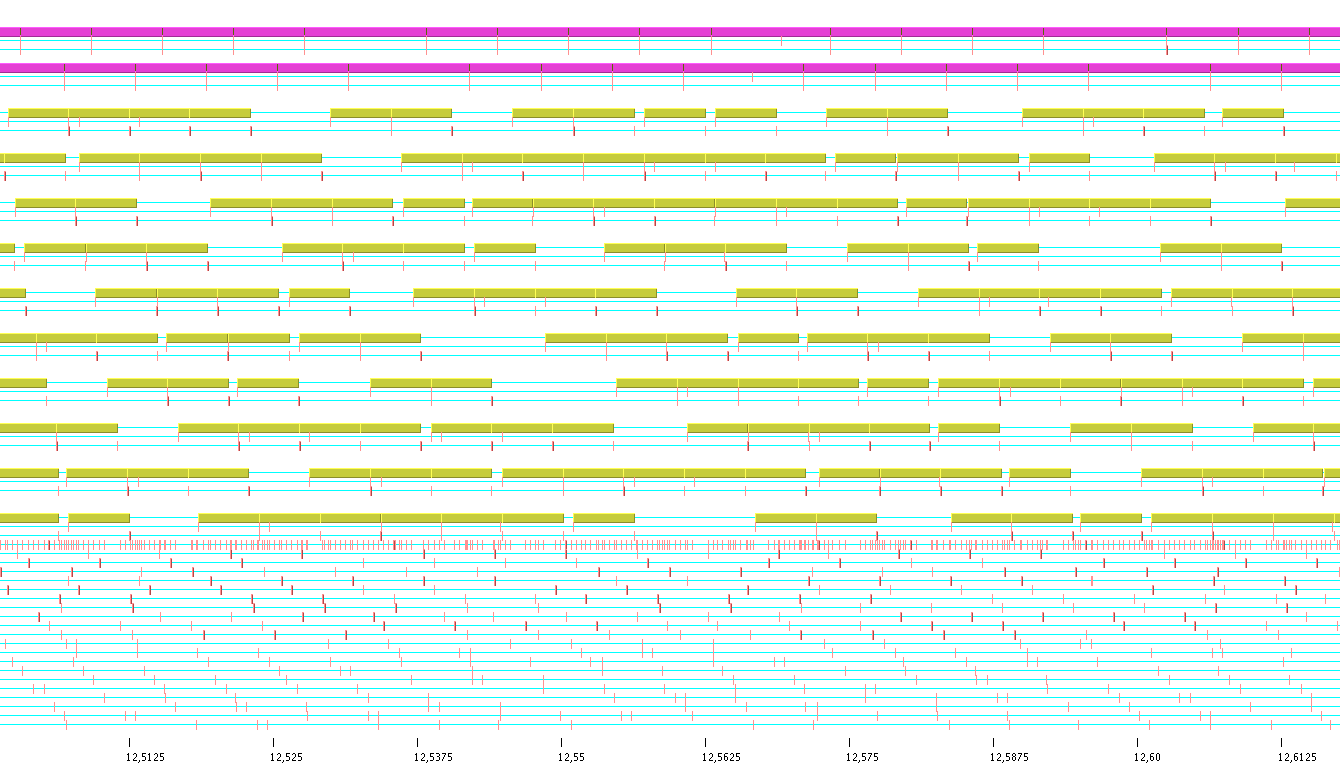
\includegraphics[width=\textwidth]{images/Screenshot-IndividualLater-5KB-1OpPerIteration.png}
}

\frame{
 \begin{block}{These}
  I/O Anfragen der 10 Clients sind später über die 10 Server verteilt\\
  $\Rightarrow$ Keine Aggregation auf den Servern möglich
 \end{block}
 \begin{block}{Prüfung}
  \begin{itemize}
   \item Test mit mehr Clients -- 100 Clients
   \item NoCache = 0.9 MB/s - (nahezu Random Zugriffe)
   \item ServerDirectedIO = 4.4 MB/s
  \end{itemize}
  \end{block}
}

\frame{
  \frametitle{Eine Iteration - 5\,KB - Unabhängige 100 Blöcke/Iteration}
        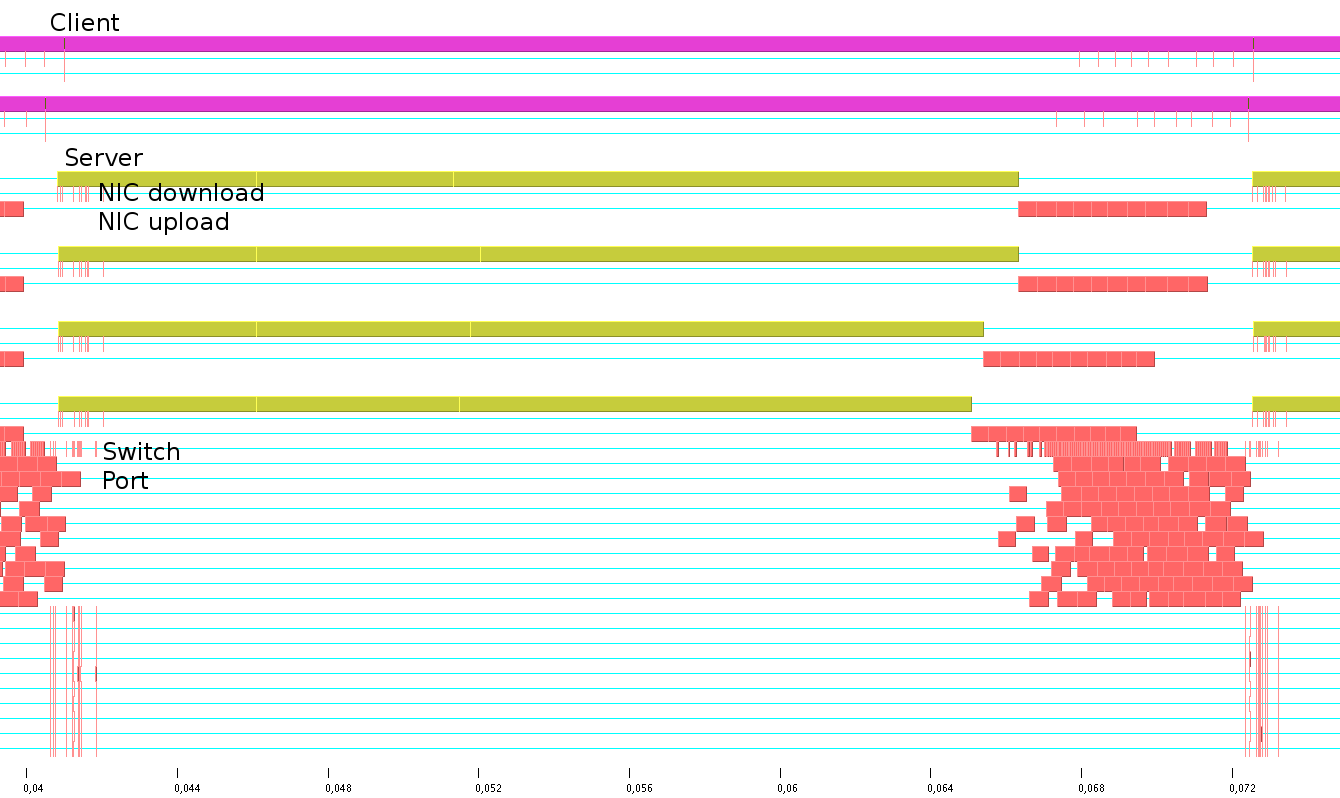
\includegraphics[width=\textwidth]{images/Screenshot-Individuall-100.png}
}

\frame{
  \begin{block}{Analyse}
  \begin{itemize}
   \item Pro Client 100 * 5\,KB = 500\,KB
   \item Durch Zugriffsmuster Clients brauchen Blöcke von jedem Server 
   \item Aggregation bündelt Anfragen sinnvoll zusammen
   \item Sobald I/O beendet ist werden alle Clients aktiv 
   \itemm{$\Rightarrow$ implizite Synchronisation}
   \item Leerzeiten auf Server
  \end{itemize}
  \end{block}
}

%Kritische Betrachtungen
%Interface für (Hardware) Komponenten teilweise schwer definierbar
%Hängt von Hardware Eigenschaften ab
%Gegenwärtig werden Interfaces nach Anforderungen erweitert
%Server Cache Layer aber soweit fest

\section{Fazit}
\myframe{Fazit}{
  \item Einfaches Model für Simulation von MPI und Cluster Hardware
  \item Geeignet für Simulation von heterogenen Umgebungen
  \item Alternative Implementierungen für MPI Befehle evaluieren
  \item Ergebnisse am Beispiel von I/O Optimierungen
  \itemm {Server-Seitige Optimierung in den vielen Fällen ausreichend}
  \item Visualisierung des Systemverhaltens vereinfacht Analyse
}
\end{document}
